\begin{figure}
\centering
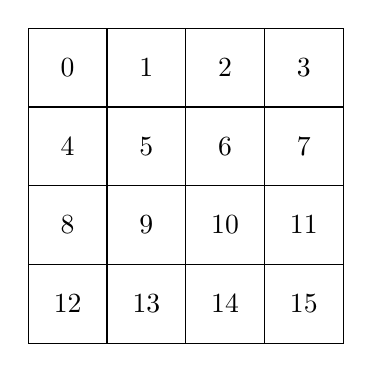
\begin{tikzpicture}
\foreach \i in {0,1,2,3}{
	\foreach \j in {0,1,2,3}{
		\draw (\i,\j) rectangle (\i+1,\j+1) ;
	}
}
\draw (.5,3.5) node {$0$};
\draw (1.5,3.5) node {$1$};
\draw (2.5,3.5) node {$2$};
\draw (3.5,3.5) node {$3$};

\draw (.5,2.5) node {$4$};
\draw (1.5,2.5) node {$5$};
\draw (2.5,2.5) node {$6$};
\draw (3.5,2.5) node {$7$};

\draw (.5,1.5) node {$8$};
\draw (1.5,1.5) node {$9$};
\draw (2.5,1.5) node {$10$};
\draw (3.5,1.5) node {$11$};

\draw (.5,.5) node {$12$};
\draw (1.5,.5) node {$13$};
\draw (2.5,.5) node {$14$};
\draw (3.5,.5) node {$15$};


\end{tikzpicture}
\caption{Numbering \yr{name figure}}
\label{fig:numbering}
\end{figure}